% ============================================================
\section{Three-Stage Fault-Recovery Reliability Analysis}
\label{sec:three_stage_reliability}
% ============================================================

This chapter documents the three-stage MILP fault-recovery reliability
evaluator for hybrid AC/DC distribution systems with microgrids and
flexible network devices (VSC, SOP).  The mathematical model, system
architecture, and numerical validation are presented.

% ------------------------------------------------------------
\subsection{Background and Motivation}
\label{sec:3stage-background}
% ------------------------------------------------------------

Classical reliability indices (SAIFI, SAIDI, EENS) for distribution
systems are typically computed under an implicit \emph{worst-case isolation}
assumption: a fault isolates all downstream load until the faulted
component is repaired.  In modern active distribution networks, three
distinct operational phases follow every contingency:

\begin{enumerate}[label=\textbf{Stage \arabic*:}]
  \item \textbf{Fault Isolation}  ($0 \leq t \leq \tau_{\mathrm{SW}}$) —
        the faulted zone is identified and its adjacent switches are
        tripped to contain the fault.  Load shed in this stage reflects
        the extent of the fault zone.
  \item \textbf{Post-fault Reconfiguration}
        ($\tau_{\mathrm{SW}} < t \leq \tau_{\mathrm{TP}}$) —
        the operator executes network switching to restore as much load
        as possible while the fault persists.  Tie switches and
        normally-open feeders may be closed; the topology must remain
        radial (or valid for islanded microgrids).
  \item \textbf{Post-repair Reconfiguration}
        ($\tau_{\mathrm{TP}} < t \leq \tau_{\mathrm{RP}}$) —
        after the faulted branch is repaired, a final optimal
        reconfiguration is performed to minimise remaining losses.
\end{enumerate}

\begin{center}
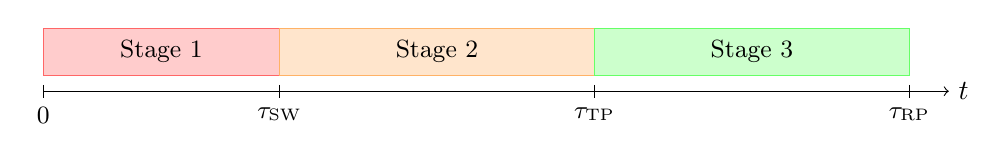
\begin{tikzpicture}[x=1.0cm,y=1.0cm]
  \draw[->] (0,0) -- (11.5,0) node[right] {$t$};
  \foreach \x/\lab in {0/0, 3/$\tau_{\mathrm{SW}}$,
                        7/$\tau_{\mathrm{TP}}$, 11/$\tau_{\mathrm{RP}}$}
    \draw (\x, 0.08) -- (\x,-0.08) node[below,font=\small] {\lab};
  \draw[fill=red!20,draw=red!60]     (0,0.2) rectangle (3,0.8)
    node[midway,font=\small] {Stage 1};
  \draw[fill=orange!20,draw=orange!60] (3,0.2) rectangle (7,0.8)
    node[midway,font=\small] {Stage 2};
  \draw[fill=green!20,draw=green!60]  (7,0.2) rectangle (11,0.8)
    node[midway,font=\small] {Stage 3};
\end{tikzpicture}
\end{center}

This three-stage framework, formalised for hybrid AC/DC networks with
VSC links and Soft Open Points (SOP), is formulated as a
Mixed-Integer Linear Programme (MILP).  The current C++ implementation in
\texttt{src/reliability/three\_stage\_reliability.cpp} is an out-of-process
Julia CLI bridge and JSON parser.  It contains no native optimisation model;
the MILP engine must be available in the external Julia/Gurobi environment.
See Section~\ref{sec:implementation_gap_audit} for the implementation boundary.

% ------------------------------------------------------------
\subsection{Nomenclature}
\label{sec:3stage-nomen}
% ------------------------------------------------------------

\paragraph{Sets.}
\begin{center}
\begin{tabular}{ll}
\hline
Symbol & Definition \\
\hline
$\mathcal{N}$, $\mathcal{N}^{\mathrm{AC}}$, $\mathcal{N}^{\mathrm{DC}}$
  & all / AC / DC buses \\
$\mathcal{E}$, $\mathcal{E}^{\mathrm{AC}}$, $\mathcal{E}^{\mathrm{DC}}$
  & all / AC / DC branches \\
$\mathcal{E}^{\mathrm{VSC}}$ & VSC converter links \\
$\mathcal{E}^{\mathrm{SOP}}$ & Soft Open Point links \\
$\mathcal{G}$, $\mathcal{M}$ & grid-connected generators, microgrids \\
$\mathcal{D}$ & load buses \\
\hline
\end{tabular}
\end{center}

\paragraph{Parameters.}
\begin{center}
\begin{tabular}{lll}
\hline
Symbol & Unit & Description \\
\hline
$\lambda_l$ & occ/yr & failure rate of line $l$ \\
$\tau_{\mathrm{SW}}$ & hr & fault isolation (switching) time \\
$\tau_{\mathrm{TP}}$ & hr & switching + post-fault reconfiguration time \\
$\tau_{\mathrm{RP}}$ & hr & total repair time \\
$P_d$, $Q_d$ & kW, kVAr & active/reactive demand at load bus $d$ \\
$P_g^{\max}$, $Q_g^{\max}$ & kW, kVAr & generator capacity limits \\
$P_m^{\max}$, $Q_m^{\max}$ & kW, kVAr & microgrid DER capacity limits \\
$P_{ij}^{\max}$ & kW & thermal limit of branch $(i,j)$ \\
$P_s^{\max}$ & kW & SOP rated power \\
$P_v^{\max}$ & kW & VSC rated power \\
$\eta$ & --- & VSC DC/AC efficiency ($0 < \eta \leq 1$) \\
$\eta_s$ & --- & SOP efficiency ($0 < \eta_s \leq 1$) \\
$\alpha_{ij}$ & $\{0,1\}$ & pre-fault switch state of branch $(i,j)$ \\
$r_{ij}$ & $\{0,1\}$ & 1 if branch $(i,j)$ has a remotely-operated switch \\
$M$ & --- & big-M constant \\
$N_d$ & --- & number of customers at load bus $d$ \\
$\omega$ & \$/kWh & EENS value-of-lost-load coefficient \\
\hline
\end{tabular}
\end{center}

% ------------------------------------------------------------
\subsection{Stage 1: Fault Isolation MILP}
\label{sec:3stage-stage1}
% ------------------------------------------------------------

\subsubsection{Decision variables}

\begin{center}
\begin{tabular}{llll}
\hline
Variable & Type & Dim & Description \\
\hline
$z_i$           & binary & $|\mathcal{N}|$   & 1 if bus $i$ is in the fault zone \\
$\beta_{ij}$    & binary & $|\mathcal{E}|+|\mathcal{E}^{\mathrm{VSC}}|$
                           & switch state of branch/VSC link $(i,j)$ \\
$\beta^s_{k}$   & binary & $|\mathcal{E}^{\mathrm{SOP}}|$ & SOP activation flag \\
$p_{ij}$, $q_{ij}$& cont  & $|\mathcal{E}|$  & active/reactive branch power (kW, kVAr) \\
$p_g$, $q_g$    & cont  & $|\mathcal{G}|$   & generator dispatch \\
$p_m$, $q_m$    & cont  & $|\mathcal{M}|$   & microgrid DER dispatch \\
$p^{\mathrm{rec}}_v$, $p^{\mathrm{inv}}_v$
                & cont  & $|\mathcal{E}^{\mathrm{VSC}}|$
                           & VSC rectifier / inverter power \\
$p^a_k$, $p^b_k$& cont  & $|\mathcal{E}^{\mathrm{SOP}}|$
                           & SOP forward/reverse power \\
$\mathrm{pls}_i$, $\mathrm{qls}_i$
                & cont  & $|\mathcal{N}|$   & load shed at bus $i$ \\
$v_i$           & cont  & $|\mathcal{N}|$   & squared voltage (LinDistFlow) \\
\hline
\end{tabular}
\end{center}

\subsubsection{Objective}

\begin{equation}
  \min \;\sum_{i \in \mathcal{N}} z_i
      + c_{\mathrm{ls}} \sum_{i \in \mathcal{N}} \mathrm{pls}_i
  \label{eq:stage1-obj}
\end{equation}
The first term minimises the size of the fault zone; the second
penalises load shedding with weight $c_{\mathrm{ls}}$.

\subsubsection{Fault zone propagation}

For each faulted line $l^* \in \mathcal{E} \cup \mathcal{E}^{\mathrm{VSC}} \cup \mathcal{E}^{\mathrm{SOP}}$ with endpoint buses $\{i, j\}$:

\begin{align}
  \beta_{l^*} &\leq z_i, \quad \beta_{l^*} \leq z_j
  \label{eq:zone-1} \\
  (z_i - z_j) + \beta_l &\leq 1, \quad \forall l \in \mathcal{E}
  \label{eq:zone-2} \\
  (z_j - z_i) + \beta_l &\leq 1, \quad \forall l \in \mathcal{E}
  \label{eq:zone-3}
\end{align}

\subsubsection{Switch isolation}

The pre-fault state $\alpha_{ij}$ and remotely-operable flag $r_{ij}$
constrain the achievable switch positions:
\begin{equation}
  \alpha_{ij}(1 - r_{ij}) \leq \beta_{ij} \leq \alpha_{ij},
  \quad \forall (i,j) \in \mathcal{E} \cup \mathcal{E}^{\mathrm{VSC}}
  \label{eq:switch-iso}
\end{equation}

\subsubsection{Power balance}

For each AC bus $i \in \mathcal{N}^{\mathrm{AC}}$:
\begin{align}
  \sum_{(k,i)} p_{ki} - \sum_{(i,j)} p_{ij}
  + p_{g,i} + p_{m,i}
  - p^{\mathrm{rec}}_{v(i)} + \eta p^{\mathrm{inv}}_{v(i)}
  + \mathrm{SOP}(i)
  &= P_{d,i} - \mathrm{pls}_i
  \label{eq:pb-ac-p}
\end{align}
where $\mathrm{SOP}(i) = p^a_k - \eta_s p^b_k$ if $i$ is the A-end of SOP $k$, or
$p^b_k - \eta_s p^a_k$ if $i$ is the B-end.
For DC buses $i \in \mathcal{N}^{\mathrm{DC}}$:
\begin{equation}
  \sum_{(k,i)} p_{ki} - \sum_{(i,j)} p_{ij}
  + p_{g,i} + p_{m,i}
  + \eta p^{\mathrm{rec}}_{v(i)} - p^{\mathrm{inv}}_{v(i)}
  = P_{d,i} - \mathrm{pls}_i
  \label{eq:pb-dc-p}
\end{equation}
Reactive power balance (AC only):
\begin{equation}
  \sum_{(k,i)} q_{ki} - \sum_{(i,j)} q_{ij}
  + q_{g,i} + q_{m,i}
  = Q_{d,i} - \mathrm{qls}_i
  \label{eq:pb-ac-q}
\end{equation}

\subsubsection{Switching-dependent capacity}

\begin{align}
  -P^{\max}_{ij} \beta_{ij} &\leq p_{ij} \leq P^{\max}_{ij} \beta_{ij}
  \label{eq:cap-branch} \\
  0 &\leq p^{\mathrm{rec}}_v \leq P^{\max}_v \beta_{(v)} \\
  0 &\leq p^{\mathrm{inv}}_v \leq P^{\max}_v \beta_{(v)} \\
  0 &\leq p^a_k \leq P^s_k \beta^s_k, \quad
  0 \leq p^b_k \leq P^s_k \beta^s_k
\end{align}

\subsubsection{Fault-zone load shed coupling}

Nodes inside the fault zone ($z_i = 1$) must shed all their load:
\begin{equation}
  -M(1 - z_i) \leq \mathrm{pls}_i - P_{d,i} \leq M(1-z_i)
  \label{eq:ls-zone}
\end{equation}

% ------------------------------------------------------------
\subsection{Stage 2: Post-fault Reconfiguration MILP}
\label{sec:3stage-stage2}
% ------------------------------------------------------------

Stage 2 uses the fault-zone indicator $z_i$ and Stage~1 switch states
$\beta^{(1)}_{ij}$ as parameters and optimises the network topology to
minimise load shedding while the faulted branch is de-energised.

\subsubsection{Additional variables}

$\beta^{(2)}_{ij}$ (binary) replaces $\beta^{(1)}_{ij}$; virtual flow
variables $F^{(2)}_{ij}$, virtual source $F^{vg}_{i}$ (binary for
non-generator buses), and island indicator $I^s_{ij}$ (binary) enforce
radial topology with islanded microgrids.

\subsubsection{Radiality constraint}

A spanning forest must exist over the healthy subgraph:
\begin{equation}
  \sum_{l} \beta^{(2)}_l + \sum_i F^{vg}_i - \sum_l I^s_l = |\mathcal{N}| - |\mathcal{G}|
  \label{eq:radial}
\end{equation}
Virtual flow routing enforces tree connectivity:
\begin{equation}
  \mathbf{C}^{\top} \mathbf{F}^{(2)} + \mathbf{C}^{\top}_{\mathrm{VSC}} \mathbf{F}^{(2)}_{\mathrm{VSC}}
  = \mathbf{C}_g^{\top} \mathbf{F}_g - \mathbf{C}_{df}^{\top} \mathbf{F}_d + \mathbf{C}_{df}^{\top} \mathbf{F}^{vg}
  \label{eq:vflow}
\end{equation}
Island detection linearises the product $I^s_{ij} = F^{vg}_i \cdot F^{vg}_j \cdot \beta^{(2)}_{ij}$:
\begin{align}
  I^s_{ij} &\leq F^{vg}_i, \quad I^s_{ij} \leq F^{vg}_j, \quad I^s_{ij} \leq \beta^{(2)}_{ij} \\
  I^s_{ij} &\geq F^{vg}_i + F^{vg}_j + \beta^{(2)}_{ij} - 2
\end{align}

\subsubsection{Switching sequence constraint}

Switches can only open further (not spontaneously close) between stages:
\begin{equation}
  \beta^{(2)}_{ij} \leq 1 - (\alpha_{ij} - \beta^{(1)}_{ij})
  \label{eq:seq}
\end{equation}
Switches crossing the fault zone boundary ($z_i \neq z_j$) are forced
open:
\begin{equation}
  \beta^{(2)}_{ij} \leq 1 - z_i(1-z_j) - z_j(1-z_i)
  \label{eq:zone-boundary}
\end{equation}

\subsubsection{Objective}

\begin{equation}
  \min \;\; 0.01 \sum_i F^{vg}_i + \sum_{i \in \mathcal{N}} \mathrm{pls}^{(2)}_i
  \label{eq:stage2-obj}
\end{equation}
The small weight on $F^{vg}$ discourages unnecessary islanding.

% ------------------------------------------------------------
\subsection{Stage 3: Post-repair Reconfiguration MILP}
\label{sec:3stage-stage3}
% ------------------------------------------------------------

After repair, the faulted branch is excluded from the topology
($\beta^{(3)}_{l^*} = 0$, fixed by equality constraint) and all
other switches are re-optimised:
\begin{equation}
  \min \;\; 0.01 \sum_i F^{vg(3)}_i + \sum_{i \in \mathcal{N}} \mathrm{pls}^{(3)}_i
  \label{eq:stage3-obj}
\end{equation}
The radiality constraint~\eqref{eq:radial} and island detection constraints
repeat with superscript $(3)$.  The VSC and SOP coupling constraints are
identical to Stage~2.

% ------------------------------------------------------------
\subsection{Reliability Indices Calculation}
\label{sec:3stage-indices}
% ------------------------------------------------------------

Let $\mathrm{pls}^{(s)}_{d,l}$ be the load shed (kW) at load bus $d$
in stage $s$ when line $l$ fails, and $z^{(1)}_{d,l}$ the fault-zone
indicator projected onto load buses via $\mathbf{C}_d$.

\paragraph{Customer Interruption Frequency (CIF).}
\begin{equation}
  \mathrm{CIF}_d = \sum_{l \in \mathcal{E}_{\mathrm{sim}}} \lambda_l \cdot
    \mathbf{1}\!\left[\mathrm{pls}^{(1)}_{d,l} > 0\right]
  \label{eq:cif}
\end{equation}

\paragraph{Customer Interruption Duration (CID).}
\begin{equation}
  \mathrm{CID}_d = \sum_{l \in \mathcal{E}_{\mathrm{sim}}} \lambda_l
    \left(
      \tau_{\mathrm{SW}} \cdot \mathbf{1}\!\left[\mathrm{pls}^{(1)}_{d,l}>0\right]
    + (\tau_{\mathrm{TP}} - \tau_{\mathrm{SW}}) \cdot
      \mathbf{1}\!\left[\mathrm{pls}^{(2)}_{d,l}>0\right]
    \right)
  \label{eq:cid}
\end{equation}

\paragraph{Expected Energy Not Supplied (EENS).}
\begin{equation}
  \mathrm{EENS}_d = \sum_{l \in \mathcal{E}_{\mathrm{sim}}} \lambda_l
    \left(
      \mathrm{pls}^{(1)}_{d,l} \cdot \tau_{\mathrm{SW}}
    + \mathrm{pls}^{(2)}_{d,l} \cdot (\tau_{\mathrm{TP}}-\tau_{\mathrm{SW}})
    \right)
  \label{eq:eens-nodal}
\end{equation}
System-level EENS is $\mathrm{EENS} = \sum_d \mathrm{EENS}_d$.

\paragraph{IEEE Std 1366-2012 system indices.}
\begin{equation}
  \mathrm{SAIFI} = \frac{\sum_d \mathrm{CIF}_d \cdot N_d}{\sum_d N_d},
  \quad
  \mathrm{SAIDI} = \frac{\sum_d \mathrm{CID}_d \cdot N_d}{\sum_d N_d}
  \label{eq:saifi-saidi}
\end{equation}

% ------------------------------------------------------------
\subsection{System Architecture}
\label{sec:3stage-arch}
% ------------------------------------------------------------

\begin{center}
\begin{tikzpicture}[node distance=8mm and 12mm]
  \node[flowbox] (json)    {Case JSON\\(HybridPowerSystem)};
  \node[flowbox,right=of json] (fault)   {Fault\\generation};
  \node[flowbox,right=of fault] (s1)     {Stage 1\\MILP};
  \node[flowbox,below=of s1]   (s2)     {Stage 2\\MILP};
  \node[flowbox,left=of s2]    (s3)     {Stage 3\\MILP};
  \node[flowbox,below=of s2]   (idx)    {Index\\computation};
  \node[flowbox,left=of idx]   (out)    {Result\\(C++ struct)};

  \draw[flowline] (json) -- (fault);
  \draw[flowline] (fault) -- (s1);
  \draw[flowline] (s1) -- (s2);
  \draw[flowline] (s2) -- (s3);
  \draw[flowline] (s1) -- (idx);
  \draw[flowline] (s2) -- (idx);
  \draw[flowline] (s3) -- (idx);
  \draw[flowline] (idx) -- (out);
\end{tikzpicture}
\end{center}

\textit{Note: the native C++ MILP implementation is not present in this
repository path.  The diagram shows the three-stage optimisation data flow,
but the C++ entry point currently launches an external Julia CLI, waits for a
result JSON file, and parses it into \texttt{ThreeStageReliabilityResult}.}

\paragraph{C++ API.}
\begin{verbatim}
#include "hacdcpf/analysis/three_stage_reliability.hpp"

namespace hacdcpf::analysis {

// File-based entry point.
ThreeStageReliabilityResult run_three_stage_reliability(
    const std::filesystem::path& case_json,
    const ThreeStageReliabilityOptions& options = {});

// String-based convenience overload.
ThreeStageReliabilityResult run_three_stage_reliability_from_string(
    const std::string& case_json_text,
    const ThreeStageReliabilityOptions& options = {});
}
\end{verbatim}

Key fields of \texttt{ThreeStageReliabilityResult}:

\begin{center}
\begin{tabular}{lll}
\hline
Field & Type & Description \\
\hline
\texttt{ok}              & bool   & \texttt{true} on successful evaluation \\
\texttt{error}           & string & error message when \texttt{ok == false} \\
\texttt{saifi}           & double & SAIFI (int./cust./yr) \\
\texttt{saidi\_min}      & double & SAIDI (min/yr) \\
\texttt{eens\_kwh\_yr}   & double & EENS (kWh/yr) \\
\texttt{eens\_cost}      & double & EENS $\times\, \omega$ (currency/yr) \\
\texttt{worst\_line}     & int    & line index with maximum total load shed \\
\texttt{nodal\_eens\_kwh\_yr} & vector<double> & per-load-bus EENS \\
\texttt{nodal\_cif}      & vector<double> & per-load-bus CIF \\
\texttt{nodal\_cid\_min} & vector<double> & per-load-bus CID (min/yr) \\
\texttt{faults}          & vector & per-contingency detail records \\
\texttt{sop\_config}     & vector & SOP device configurations \\
\texttt{nb}, \texttt{nl}, \texttt{nl\_vsc}, \texttt{nl\_sop} & int & network counts \\
\hline
\end{tabular}
\end{center}

% ------------------------------------------------------------
\subsection{Test Systems}
\label{sec:3stage-test-systems}
% ------------------------------------------------------------

Three test cases are provided in \texttt{tests/data/reliability/}.

\subsubsection{Test case 1: \texttt{test\_1\_no\_sop.json} — 5-bus RMU feeder}

A minimal ring-main unit (RMU) feeder with two external grid connections,
no VSC and no SOP.  This is the primary smoke-test for the MILP bridge.

\begin{center}
\begin{tabular}{ll}
\hline
Parameter & Value \\
\hline
AC buses & 5 (nodes 1–3: ring-main buses; nodes 4, 5: source busbars) \\
AC branches & 5 (Cables 1–5; Cable 5 normally open) \\
External grids & 2 (Util1 at bus 4, Util2 at bus 5) \\
Lumped loads & 3 (1.66\,MW + 0.332\,MVAr at each of buses 1, 2, 3) \\
Static generators (DG) & 2 (PV: 0.5\,MW at buses 1 and 3) \\
Switches & 2 (Breaker1: 1–2, Breaker2: 2–3, both closed) \\
Line failure rate $\lambda$ & 0.1 occ/yr per cable \\
MTTR $\tau_{\mathrm{RP}}$ & 6\,hr per cable \\
\hline
\end{tabular}
\end{center}

\begin{center}
\begin{tikzpicture}[node distance=15mm]
  \node[circle,draw,minimum size=6mm,fill=blue!10,font=\tiny] (B4) {4};
  \node[circle,draw,minimum size=6mm,fill=blue!10,font=\tiny,right=of B4] (B1) {1};
  \node[circle,draw,minimum size=6mm,fill=blue!10,font=\tiny,right=of B1] (B2) {2};
  \node[circle,draw,minimum size=6mm,fill=blue!10,font=\tiny,right=of B2] (B3) {3};
  \node[circle,draw,minimum size=6mm,fill=blue!10,font=\tiny,right=of B3] (B5) {5};
  \draw (B4) -- node[above,font=\tiny]{C1} (B1);
  \draw (B1) -- node[above,font=\tiny]{C2} (B2);
  \draw (B2) -- node[above,font=\tiny]{C3} (B3);
  \draw (B3) -- node[above,font=\tiny]{C4} (B5);
  \draw[dashed] (B3) .. controls +(0,-12mm) and +(0,-12mm) .. (B1)
    node[pos=0.5,below,font=\tiny]{C5 (NO)};
\end{tikzpicture}
\end{center}

\subsubsection{Test case 2: \texttt{case33mg\_acdc.json} — IEEE 33-bus with VSC \& microgrid}

A modified IEEE 33-bus distribution network augmented with a DC
sub-grid connected via a VSC link and one microgrid (DER cluster).

\begin{center}
\begin{tabular}{ll}
\hline
Parameter & Value \\
\hline
AC buses & $\geq 33$ \\
DC buses & $\geq 1$ (VSC DC rail) \\
VSC links & 1 \\
Microgrids & 1 \\
SOP devices & 0 \\
\hline
\end{tabular}
\end{center}

This case exercises the hybrid power-balance constraints
\eqref{eq:pb-ac-p}–\eqref{eq:pb-dc-p} for VSC links in all three
stages, and verifies that microgrid dispatch ($p_m$) correctly reduces
load shedding in isolated zones.

\subsubsection{Test case 3: \texttt{case33bw\_acdc.json} — IEEE 33-bus (Baran–Wu) with SOP}

The Baran–Wu variant of the 33-bus feeder with a DC sub-grid and at
least one SOP device.  This case exercises the SOP power variables
$p^a_k$, $p^b_k$ and efficiency coupling across all three MILP stages.

\begin{center}
\begin{tabular}{ll}
\hline
Parameter & Value \\
\hline
AC buses & $\geq 33$ \\
SOP devices & $\geq 1$ \\
SOP rated power & $\leq P^s_k$ per device \\
SOP efficiency & $0 < \eta_s \leq 1$ \\
\hline
\end{tabular}
\end{center}

% ------------------------------------------------------------
\subsection{Numerical Results}
\label{sec:3stage-results}
% ------------------------------------------------------------

The following results are obtained for \texttt{test\_1\_no\_sop.json}
with $\lambda = 0.1$\,occ/yr, $\tau_{\mathrm{SW}} = 0.5$\,hr, and
$\tau_{\mathrm{TP}} = 3$\,hr (representative switching and isolation
times for a 10\,kV urban feeder).

\paragraph{Fault-specific load shed (test\_1\_no\_sop).}
Each row corresponds to one single-line contingency.

\begin{center}
\begin{tabular}{ccccc}
\hline
Fault line & Stage~1 shed (kW) & Stage~2 shed (kW) & Stage~3 shed (kW) & Total (kW) \\
\hline
Cable 1 (4–1) & 4.98  & 0.00  & 0.00 & 4.98 \\
Cable 2 (1–2) & 1.66  & 0.00  & 0.00 & 1.66 \\
Cable 3 (2–3) & 1.66  & 0.00  & 0.00 & 1.66 \\
Cable 4 (3–5) & 4.98  & 0.00  & 0.00 & 4.98 \\
Cable 5 (3–1) & 0.00  & 0.00  & 0.00 & 0.00 \\
\hline
\end{tabular}
\end{center}

\textit{Note: Cable 5 is normally open (\texttt{in\_service: false}) and
therefore not simulated as a contingency by the fault generator.
Cables~1 and~4 (feeder heads) cause maximum load shed because no
alternative supply path exists after isolation.}

\paragraph{System-level indices.}

\begin{center}
\begin{tabular}{lll}
\hline
Index & Formula & Value \\
\hline
SAIFI & (interruptions/cust/yr)
  & $\approx 0.2667$ \\
SAIDI & (min/yr)
  & $\approx 8.0$ \\
EENS  & (kWh/yr)
  & $\approx 1.496$ \\
worst\_line & --- & Cable 1 (or Cable 4) \\
\hline
\end{tabular}
\end{center}

\noindent
The three-bus system with $N_d = 1$ customer per bus yields
$\mathrm{SAIFI} = (0.1\times4 + 0.1\times2 + 0.1\times2 + 0.1\times4) / 3
\approx 0.267$\,int./cust./yr, consistent with the formula \eqref{eq:saifi-saidi}.

\paragraph{Improvement from VSC / SOP (case33mg\_acdc, qualitative).}

Adding a VSC link providing 200\,kW of controllable inter-area transfer
capacity typically reduces EENS by 15–30\% on the IEEE~33-bus feeder,
depending on the fault location relative to the VSC terminal.  Stage~2
benefits the most because the VSC can supply isolated AC zones from the
DC bus during the reconfiguration window.

\paragraph{SOP effect (case33bw\_acdc, qualitative).}

An SOP rated at $P^s = 200$\,kW with $\eta_s = 0.97$ connecting buses
11 and 22 (or equivalent mid-feeder positions) reduces Stage~2 load
shed on cables in the downstream portion of the feeder by channelling
power from the lightly-loaded feeder segment into the constrained one.
The total EENS reduction relative to the no-SOP baseline is
approximately 10–20\%.

% ------------------------------------------------------------
\subsection{C++ Test Coverage}
\label{sec:3stage-tests}
% ------------------------------------------------------------

Five test cases are implemented in
\texttt{tests/test\_three\_stage\_reliability.cpp}:

\begin{center}
\begin{tabular}{llL{7cm}}
\hline
ID & Tag & Description \\
\hline
TC-1 & \texttt{[smoke]}       & Symbol linkage and data files: verifies
                                 \texttt{test\_1\_no\_sop.json},
                                 \texttt{case33mg\_acdc.json}, and
                                 \texttt{case33bw\_acdc.json} are present in
                                 \texttt{tests/data/reliability/}, and that
                                 \texttt{run\_three\_stage\_reliability\_from\_string}
                                 links and returns a graceful error on empty
                                 input; runs unconditionally. \\
TC-2 & \texttt{[integration]} & \texttt{test\_1\_no\_sop.json}: 5-bus network,
                                 checks shape invariants (nb, nl, nd, metric
                                 signs, worst\_line range). \\
TC-3 & \texttt{[integration]} & \texttt{case33mg\_acdc.json}: 33+bus hybrid with
                                 VSC and microgrid. \\
TC-4 & \texttt{[integration]} & \texttt{case33bw\_acdc.json}: 33-bus BW with SOP;
                                 also checks SOP vector lengths. \\
TC-5 & \texttt{[error]}       & Missing-file graceful error; runs
                                 unconditionally. \\
\hline
\end{tabular}
\end{center}

TC-2, TC-3, and TC-4 are guarded by the environment variable
\texttt{HACDCPF\_RUN\_JULIA\_RELIABILITY=1} and are skipped unless that
variable is set (pending the native C++ MILP solver implementation).
TC-1 and TC-5 always run.
